\section{Background}
\label{sec:background}


\begin{figure}[!tb]
  \center
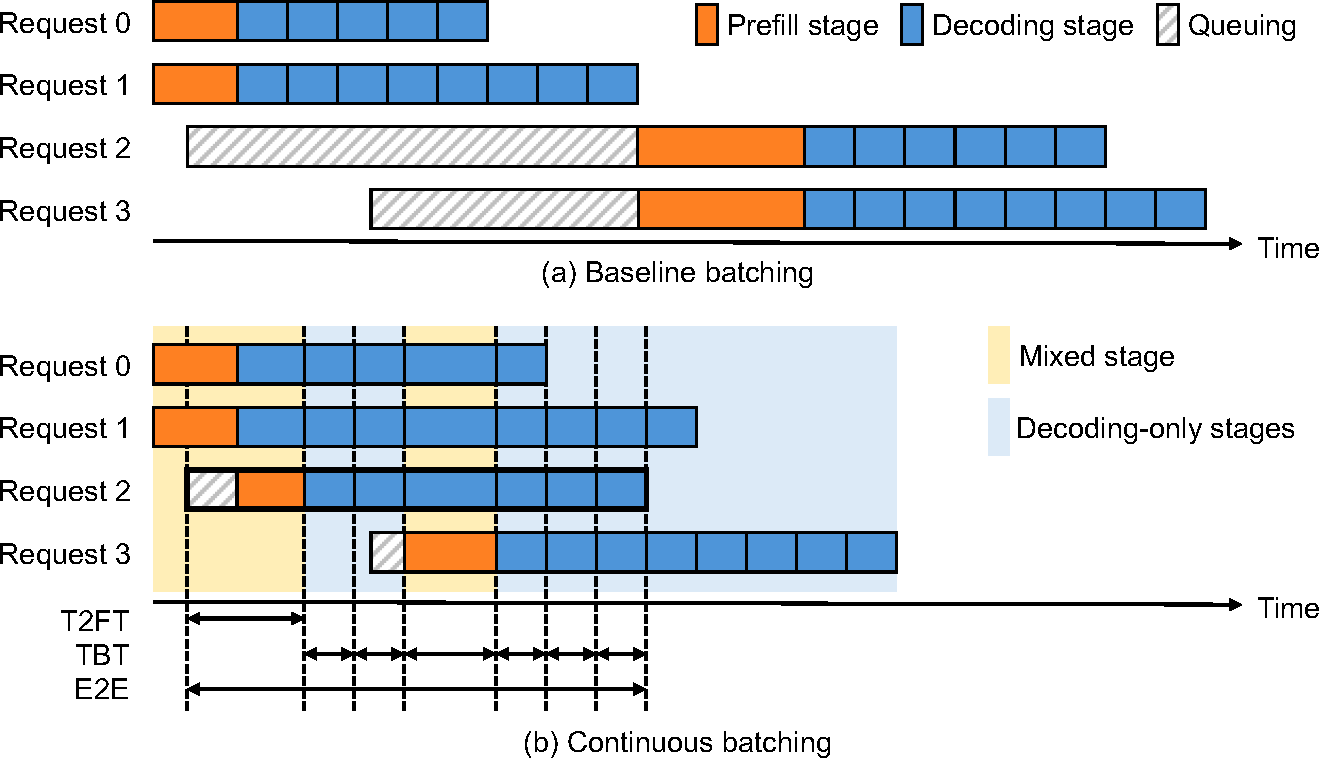
\includegraphics[width=1.0\columnwidth]{figures/scheduling.pdf}
  \caption{
  (a) Baseline batching, which performs inference at the request level. (b) Continuous batching, which performs inference at the stage level. \ttft, \tbt, and \ete latency values for request 2 are also detailed.
  }
  \label{fig:scheduling}
  \vspace{-0.05in}
\end{figure}

\subsection{Structure of Large Language Models (LLMs)}
\label{sec:background:structure}
Most recently proposed LLMs consist of decoders originally introduced for the transformer model~\cite{neurips_2017_transformer}.
An LLM features sequentially stacked (connected) decoder blocks with a token embedding layer at the beginning and a language modeling (LM) head layer at the end (see Fig.~\ref{fig:llm_model}), where a token is the unit of interpretation.
Upon receiving an inference request expressed as a sequence of tokens, each token is first transformed into a hidden vector with dimensions ranging from thousands to tens of thousands by the token embedding layer.
Hereafter, we refer to the hidden vectors as tokens.
The following decoder block comprises a multi-head attention (MHA) layer, a feed-forward network (FFN) layer, and several other layers that are relatively lightweight from a computational perspective.

MHA first generates query (Q), key (K), and value (V) matrices or vectors from the input sequence through fully-connected (FC) operations.
Each of Q, K, and V is partitioned into evenly sized slices, distributed to \nhead heads (Q\textsubscript{i}, K\textsubscript{i}, and V\textsubscript{i} for i = 0, 1, ..., \nhead$-1$), in which an attention operation is performed.
For each head, a Q slice is multiplied with a K slice, softmax is applied, and the result is multiplied with a V slice.
Finally, projection, another FC layer, is performed for the concatenated results from the heads.
The following FFN layer consists of three FC layers with a gated activation operation (\eg, SiLU~\cite{arxiv-2023-llama2, arxiv-2024-mixtral}) in between.
We assume the use of FP16 format for the data vectors and weights in LLM inference, following conventional practices~\cite{openai-fp16, arxiv-2022-opt}.





\subsection{Mixture of Experts and Grouped-Query Attention}
\label{sec:background:moe_gqa}


To further scale the size of LLMs, hyperscalers, such as OpenAI, Google, Meta, and Microsoft, have employed model variants such as mixture of experts (MoE)~\cite{jmlr-2022-switchtransformer, emnlp-2022-metamoe, icml-2022-DSMoE, arxiv-2024-mixtral, grok1} and grouped-query attention (GQA)~\cite{emnlp-2023-gqa, arxiv-2023-llama2, arxiv-2024-mixtral, grok1}.




MoE improves the output quality while suppressing the increase in the number of operations.
MoE places multiple instances (called experts) of an FFN layer, which already accounts for the majority (about \sfrac{2}{3}) of parameters in non-MoE LLMs.
We denote the number of experts in an MoE layer as \Numex.
A gate placed at the front assigns tokens to different \topk experts; the selected experts are determined based on the input token.
Each token passes through \topk experts, and the final result of the MoE layer is obtained by the weighted summation of each \topk expert's output. 
The memory capacity requirement substantially increases to store the \Numex expert FFNs, and the bandwidth requirement also increases to access the parameters for the selected expert FFNs. 
However, the number of operations is almost the same or slightly larger than that of non-MoE LLMs, as each token only passes through \topk experts, not all experts.


GQA allows heads within an attention layer to form groups, each sharing K and V slices.
Then, Q slices for the heads in the group can perform attention with a form of general matrix-matrix multiplication (GEMM).
The total size of K and V decreases by a factor of \deggrp, the number of heads in a group, alleviating the memory bandwidth bottleneck.
At its extreme, all the heads in a layer can form a single group, which is referred to as multi-query attention (MQA); however, MQA is known to degrade the output quality compared to GQA~\cite{emnlp-2023-gqa, arxiv-2023-llama2}.
Hence, we do not consider MQA in this paper.


\begin{figure*}[!tb]
  \center
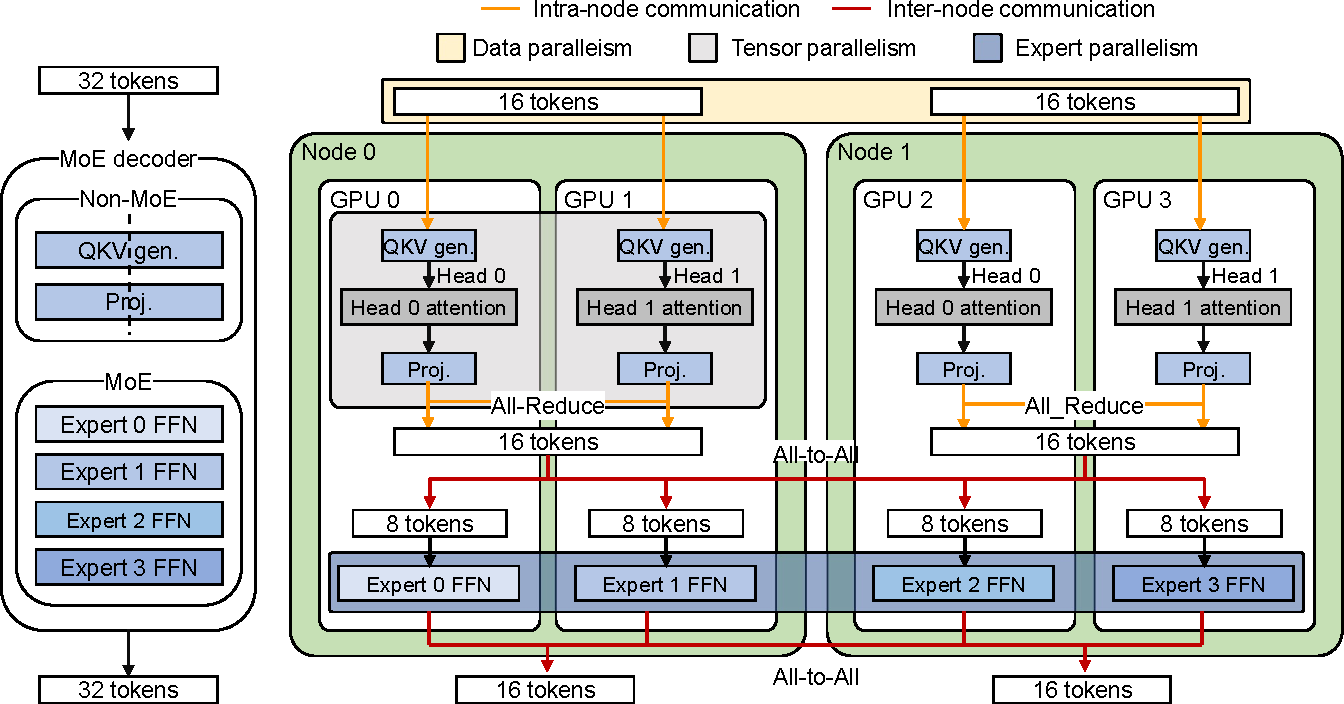
\includegraphics[width=0.70\textwidth]{figures/gpu_model_distribution.pdf}
  \vspace{-0.04in}
  \caption{
  Model distribution methodology and operation flow of an LLM in a multi-node/multi-GPU system~\cite{icml-2022-DSMoE}. For non-expert weights, systems exploit tensor parallelism in the node, and data parallelism across nodes. For expert FFNs, the system allocates each expert FFN to a different GPU.
  }
  \label{fig:gpu_distribution}
  \vspace{-0.12in}
\end{figure*}



\subsection{LLM Inference with Continuous Batching}
\label{sec:background:inference}

LLM inference involves a single prefill (summarization) stage followed by multiple decoding (generation) stages.
The former takes the entire input tokens of length $L_{in}$, passes them through the model, and generates key and value (KV) matrices as well as the first output token.
A sequence of decoding stages follows iteratively; a decoding stage receives a single output token from the previous stage and passes it through the model in a sequential manner.
Each decoding stage generates KV vectors for the input token, which are concatenated to the KV matrices, and a new output token.
Multiple decoding stages are required to constitute the output response of length $L_{out}$.

LLM inference can process multiple requests in a batch to increase serving throughput.
Both on the prefill and decoding stages, the FC layers from QKV generation, projection, and FFN layers can be batched to form GEMM operations between the batched input tokens and the weight matrices.
However, batching requests is not effective for the attention operation.
The attention operation must be performed separately for each request because the unique KV matrices corresponding to the context of each request are used.
%However, for the attention layer, batching requests is not effective as unique KV matrices corresponding to the context of each request are used.
%Instead, GEMM is performed between the Q matrix generated from the input sequence and the KV matrices in the prefill stage.
%In the decoding stage, general matrix-vector multiplication (GEMV) is performed between a single Q vector generated from the input token and the KV matrices. in the case of MHA.


To increase serving throughput, continuous batching~\cite{osdi-2022-orca} is widely used.
It divides each LLM inference into multiple stages and batches the requests at the stage level (see Fig.~\ref{fig:scheduling}(b)).
This stage-level scheduling can reduce the queuing delay of new requests and the time-to-first token (\ttft), the latency it takes for the first token to be generated upon request arrival.
We categorize each stage into the following two types depending on the presence or absence of a prefill stage request.
1) \mixedstage: prefill stages of newly added requests are batched with decoding stages of existing requests. 2) \deconlystage: all requests of a batch are in the decoding stage if there is no new request to be served at the moment a new stage starts.
We refer to the latency between two consecutive token generations as token-between-token latency (\tbt) and the request handling latency from arrival to completion as end-to-end latency (\ete).
In each stage, we refer to the requests performing decoding as decoding sequences and those performing prefill as prefill sequences.
Hereafter, batch size is determined by the number of requests in a stage.

\begin{figure*}[!tb]
  \center
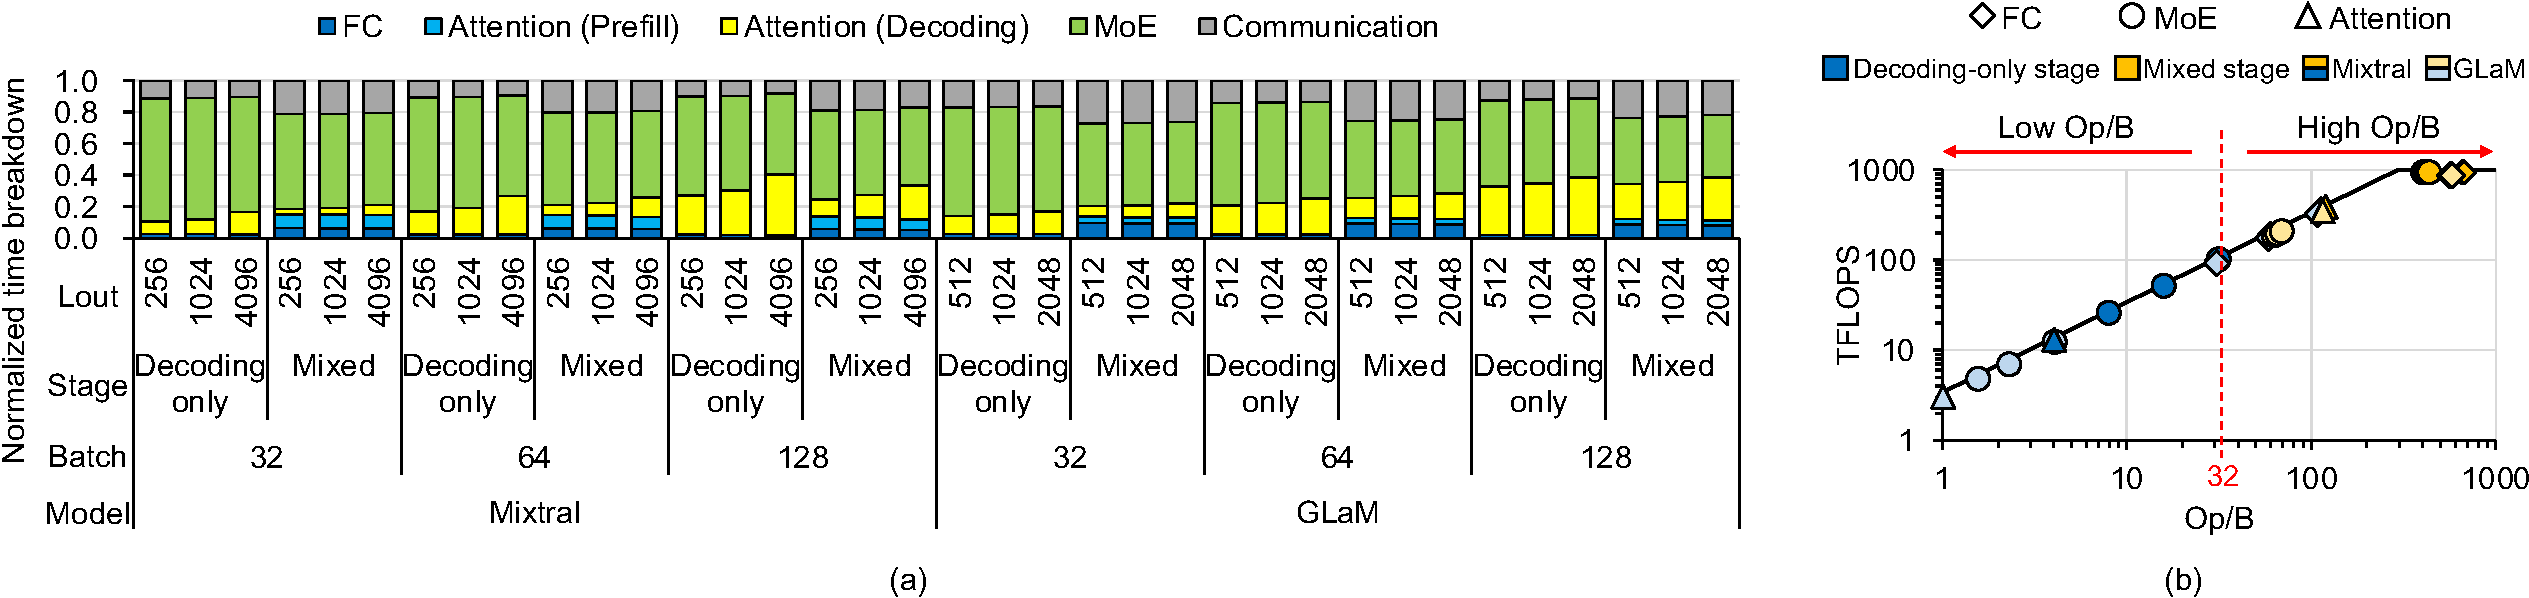
\includegraphics[width=0.95\textwidth]{figures/roofline.pdf}
  \vspace{-0.1in}
  \caption{
  (a) Execution time ratio of each operation in Mixtral~\cite{arxiv-2024-mixtral} and GLaM~\cite{icml-2022-GLaM} varying \lout and batch size while \lin = 2048. Mixtral (GLaM) uses \deggrp$=4$ $(1)$ for the attention layer and uses 8 (64) experts in the MoE layer with each token selecting the top-2 experts. (b) The roofline graph for each model on GPUs with varying batch sizes (32--128) when \lin = 2048 and \lout = 1024. Details of systems are in Section~\ref{sec:experimental_setup}.
  }
  \label{fig:roofline}
  \vspace{-0.15in}
\end{figure*}

\subsection{High Bandwidth Memory (HBM)}
\label{sec:background:hbm}
HBM has a 3D-stacked structure with one logic die at the bottom and multiple DRAM dies.
The logic die consists of I/O circuitry, memory built-in-self-test, and testing and debugging units~\cite{isca-2021-hbm-pim, pact-2018-3d-xpath}.
Through silicon vias (TSVs) connect the DRAM dies to the logic die.
We focus on 8-hi HBM3, deployed on the latest GPUs (e.g., NVIDIA H100).
In HBM3, four DRAM dies form a rank, and each DRAM die has eight pseudo channels. Each pseudo channel is connected to four bank groups of four banks, totalling 16 banks in the rank. 
The banks share external wires within a single pseudo channel, allowing them to read data from only one bank at a time.
